% \vspace{2cm}
\noindent In this chapter the results of various simulations utilising the OxDNA based
rotaxane model, discussed in Chapter 3, are presented. The aim of this computational
analysis is to shed light on
the entropic effects which play a central role in the nanopiston's operating cycle. By
extension, the thermodynamic transitions providing the free energy governing its
operation are studied.

To better understand the entropic interactions between the DNA rotaxane and the nanopore
a specially engineered rotaxane variant is studied. This other class of rotaxanes will be
called the mixed rotaxanes, as they are composed of different ds- and ssDNA fractions to
study the change in entropic interactions. Having explored the effects of the
entropic contributions, next the conformational fluctuations of the nanopiston are
simulated and analysed. Lastly, an attempt is made to simulate the thermodynamic
transitions driving the piston cycle. These particular simulations are made possible
by the use of a forward flux sampling algorithm.

% \newpage

\section{Mixed Rotaxane}



Having identified the entropic interactions as key component of the nanopiston cycle,
studying them is an important but challenging task. The problem arises when we aim to
specify the entropic contributions to the conformational fluctuations of the rotaxane.
The
main factor complicating this analysis is the multiplicity of the interactions acting
upon the nanopiston.

\begin{wrapfigure}[21]{r}{0.5\textwidth}
  \vspace{-0.8cm}
  \begin{center}
    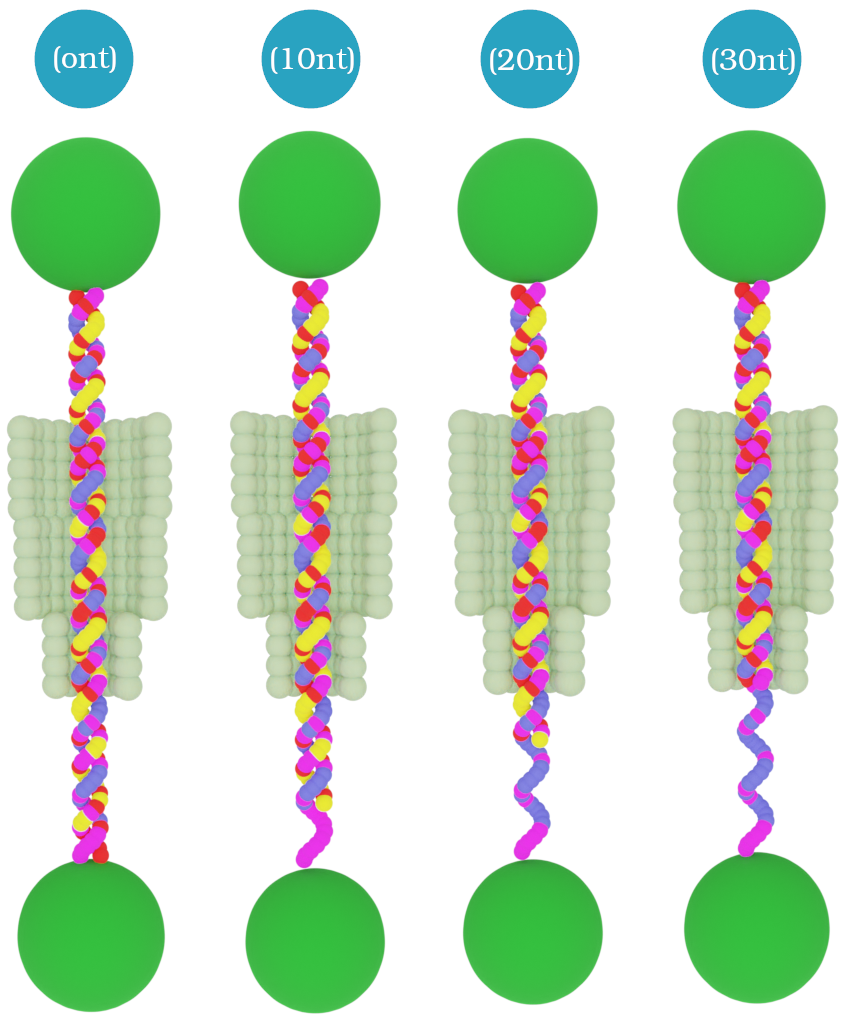
\includegraphics[width=0.4\textwidth]{Figures/mixed.png}
    \caption[Figure of the simulated mixed rotaxanes.]{{\small The different mixed
    rotaxane
    versions that are simulated. The label above the rotaxanes refers to the number of
    nucleotides (nt) that are present in the ssDNA strand of the rotaxane. Image rendered
    using Blender.\cite{blender}}}
  \label{fig:mixed}
\end{center}
\end{wrapfigure}

The first category of forces is composed of the external forces arising from the
potential difference applied over the membrane. This potential difference induces an
electric field both outside and inside of the nanopore, influencing the movement of
molecules in these regions. The most significant contributions can be identified as the
electrophoretic and electro-osmotic forces acting upon the rotaxane. The second class of
forces is composed of the intrinsic forces. These forces do not arise from the
electric field, but rather originate from the direct interactions between the rotaxane
and the nanopore itself. Under this category fall the electrostatic, steric and entropic
forces, limiting the conformational freedom of the piston.

In order to study the role of entropy in the conformational fluctuations of
the nanopiston, these effects need to be isolated from the other contributions present in
the system. To achieve this Bayoumi et al. devised a new variation of the rotaxane
called the mixed rotaxane, shown in Figure \ref{fig:mixed}. In this rotaxane variation
the ssDNA overhang is removed, resulting
in a thread composed of solely ds- and ssDNA. By varying the DNA composition of this
rotaxane the changes in entropic interactions can be analysed. More specifically, the
total length of the rotaxane was constant, i.e. the total number of nucleotides (nt) and
basepairs (bp) are fixed at 100, while the ssDNA part was varied from $0nt$ to $30 nt$ in
steps of $10nt$. The effects of these changes in composition were first studied using
experiments measuring the I-V
trace in the range of $[-100mV, +100mV]$. During an I-V measurement a range of
voltages is applied over the lipid membrane and at each step in this voltage sweep the
current through the pore is measured. A detailed explanation of this method is described
in.\cite{MAGLIA2010591} The results from these experiments are presented in Figure
\ref{fig:mixedrotaxane}a.

The mixed rotaxane composed entirely of dsDNA yields an almost linear I-V trace in the
measured voltage range, as shown in the top I-V trace of Figure \ref{fig:mixedrotaxane}a.
This result indicates a constant obstruction of the nanopore over
the entire voltage sweep. On the other hand, the mixed rotaxane composed of a $10nt$
ssDNA strand shows a drastically different I-V trace. Decreasing the voltage below
$-20mV$ results in current fluctuations between two distinct levels. A second transition
can be observed when the voltage is further decreased below $-70mV$. Here the measured
current becomes independent from the applied voltage, suggesting a partial blockage of
the current through the nanopore. These same characteristics can be identified in the I-V
trace of the mixed rotaxane with a $20nt$ ssDNA strand. Remarkably, the voltage range
in which the current fluctuations are observed is shifted to a more negative
voltage range from $-30mV$ to  $-85 mV$. In Figure \ref{fig:mixedrotaxane}a both the
blockage and the two fluctuation levels are indicated with arrows. When the fraction of
ssDNA in the mixed rotaxane is further increased to $30nt$, the characteristic blockage
is no longer observed and the linear I-V trace is recovered.

\begin{figure}[ht!]

  \begin{centering}
  \adjustbox{minipage=1.3em,valign=t}{\subcaption{}\label{sfig:testa}}%
  \begin{subfigure}[t]{\dimexpr.29\linewidth-1.3em\relax}
  \centering
  \vspace{0.35cm}
  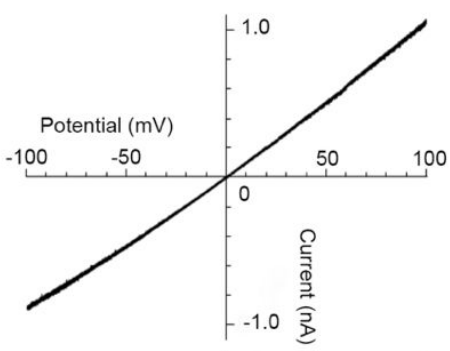
\includegraphics[width=1.05\linewidth,valign=t]{Figures/IV-100.png}
  \end{subfigure}%
  \adjustbox{minipage=1.3em,valign=t}{\subcaption{}\label{sfig:testb}}%
  \begin{subfigure}[t]{\dimexpr.46\linewidth-1.3em\relax}
  \centering
  \hspace{-0.2cm}
  \vspace{0.1cm}
  \includegraphics[width=0.95\linewidth,valign=t]{Figures/MR-100.png}
  \end{subfigure}%
  \adjustbox{minipage=1.3em,valign=t}{\subcaption{}\label{sfig:testc}}%
  \begin{subfigure}[t]{\dimexpr.21\linewidth-1.3em\relax}
  \hspace{3cm}
  \centering
  \vspace{0.2cm}
  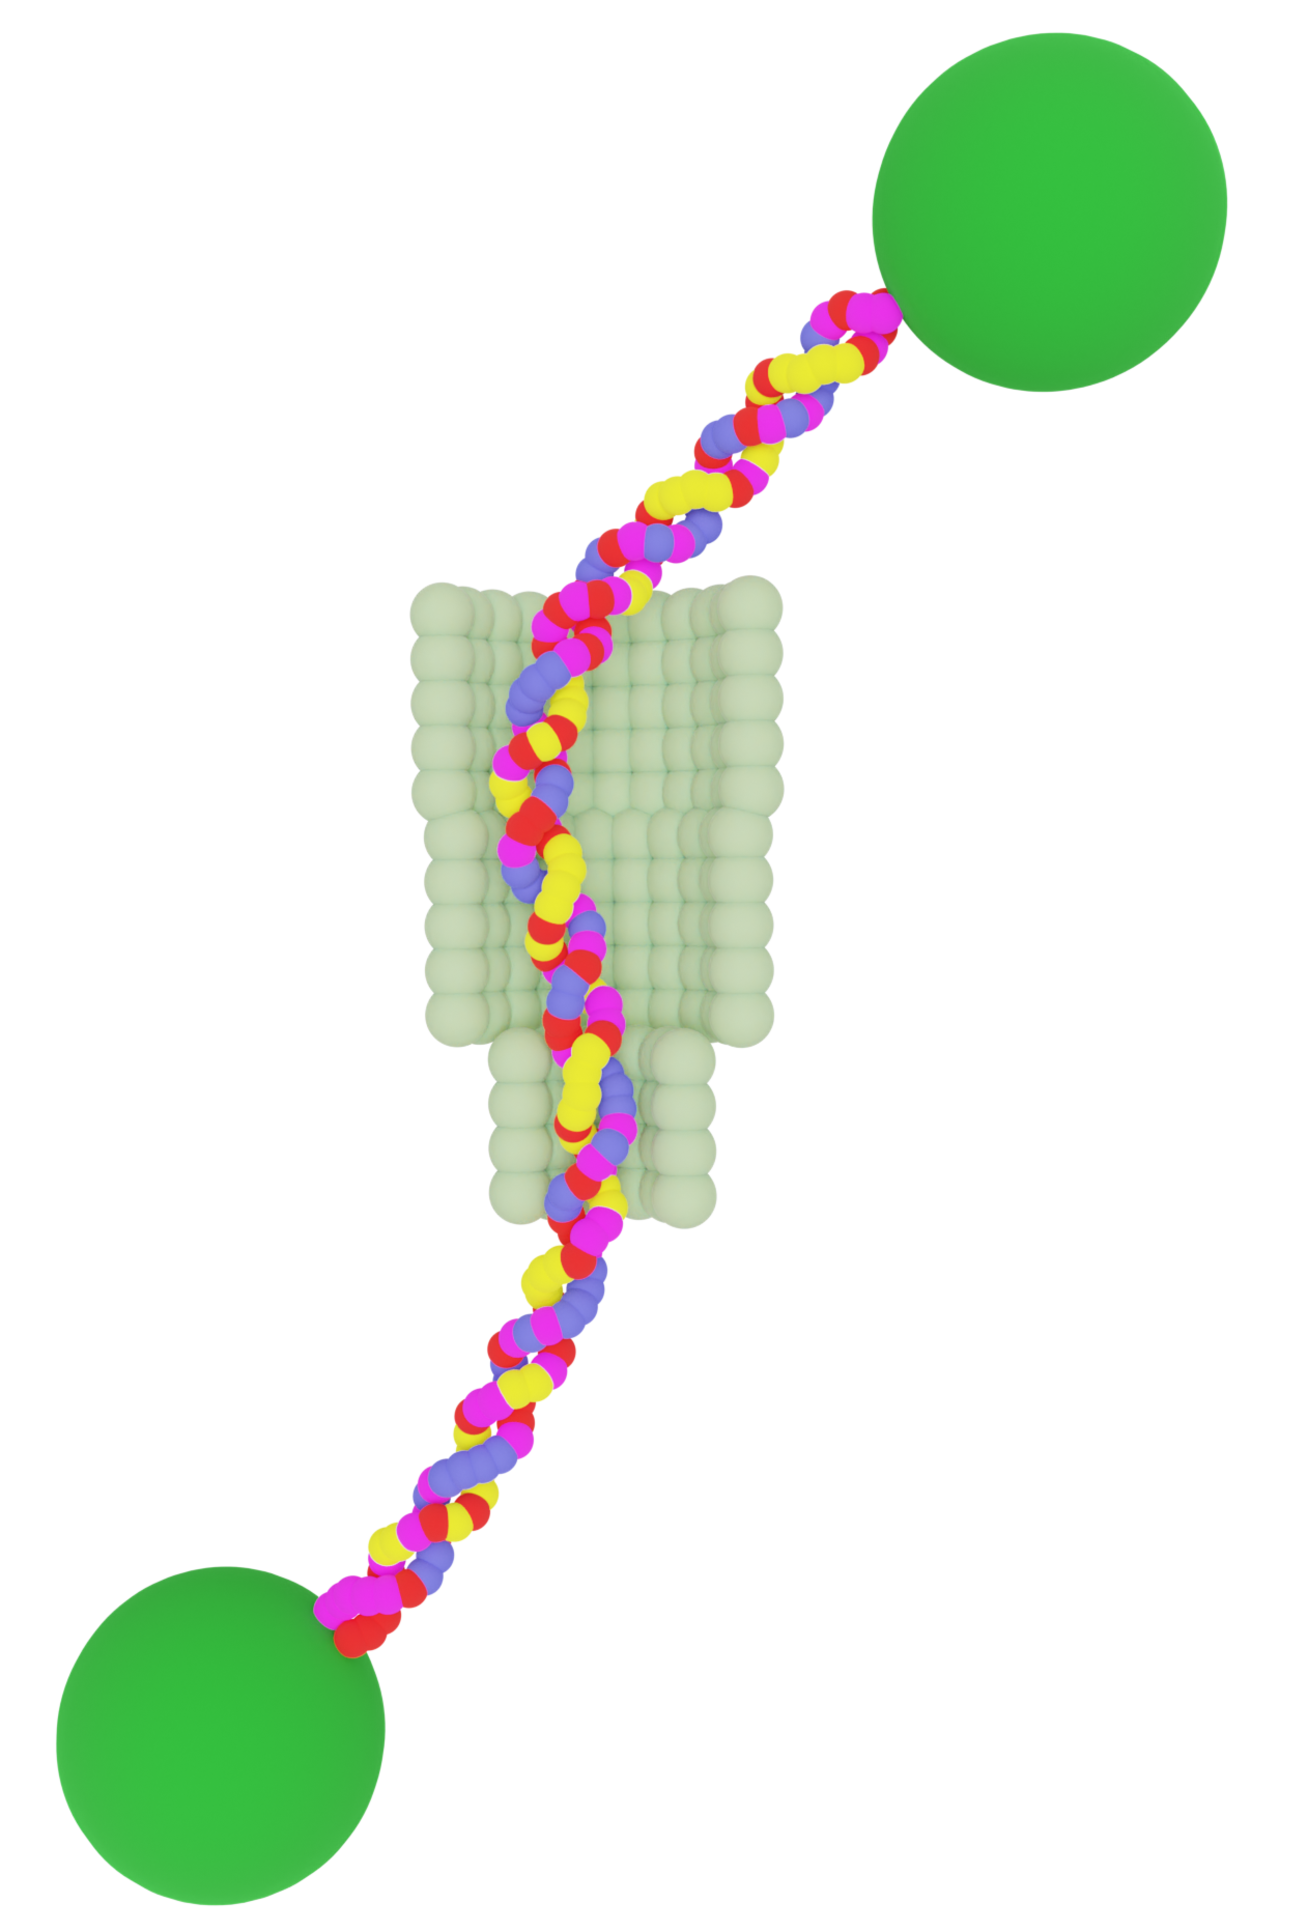
\includegraphics[width=1\linewidth,valign=t]{Figures/Rotaxane-100.png}
  \end{subfigure}
  \label{fig:test}
  \end{centering}

  \vspace{0.05cm}

  \begin{centering}
  \adjustbox{minipage=1.3em,valign=t}{}%
  \hspace{.35cm}
  \begin{subfigure}[t]{\dimexpr.3\linewidth-1.3em\relax}
  \centering
  \vspace{-0.1cm}
  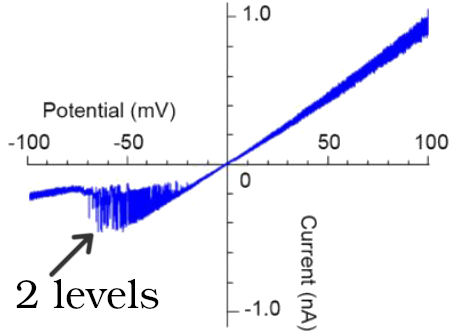
\includegraphics[width=1.05\linewidth,valign=t]{Figures/IV-90.png}
  \end{subfigure}%
  \adjustbox{minipage=1.3em,valign=t}{}%
  \hspace{.25cm}
  \vspace{-0.2cm}
  \begin{subfigure}[t]{\dimexpr.46\linewidth-1.3em\relax}
  \centering
  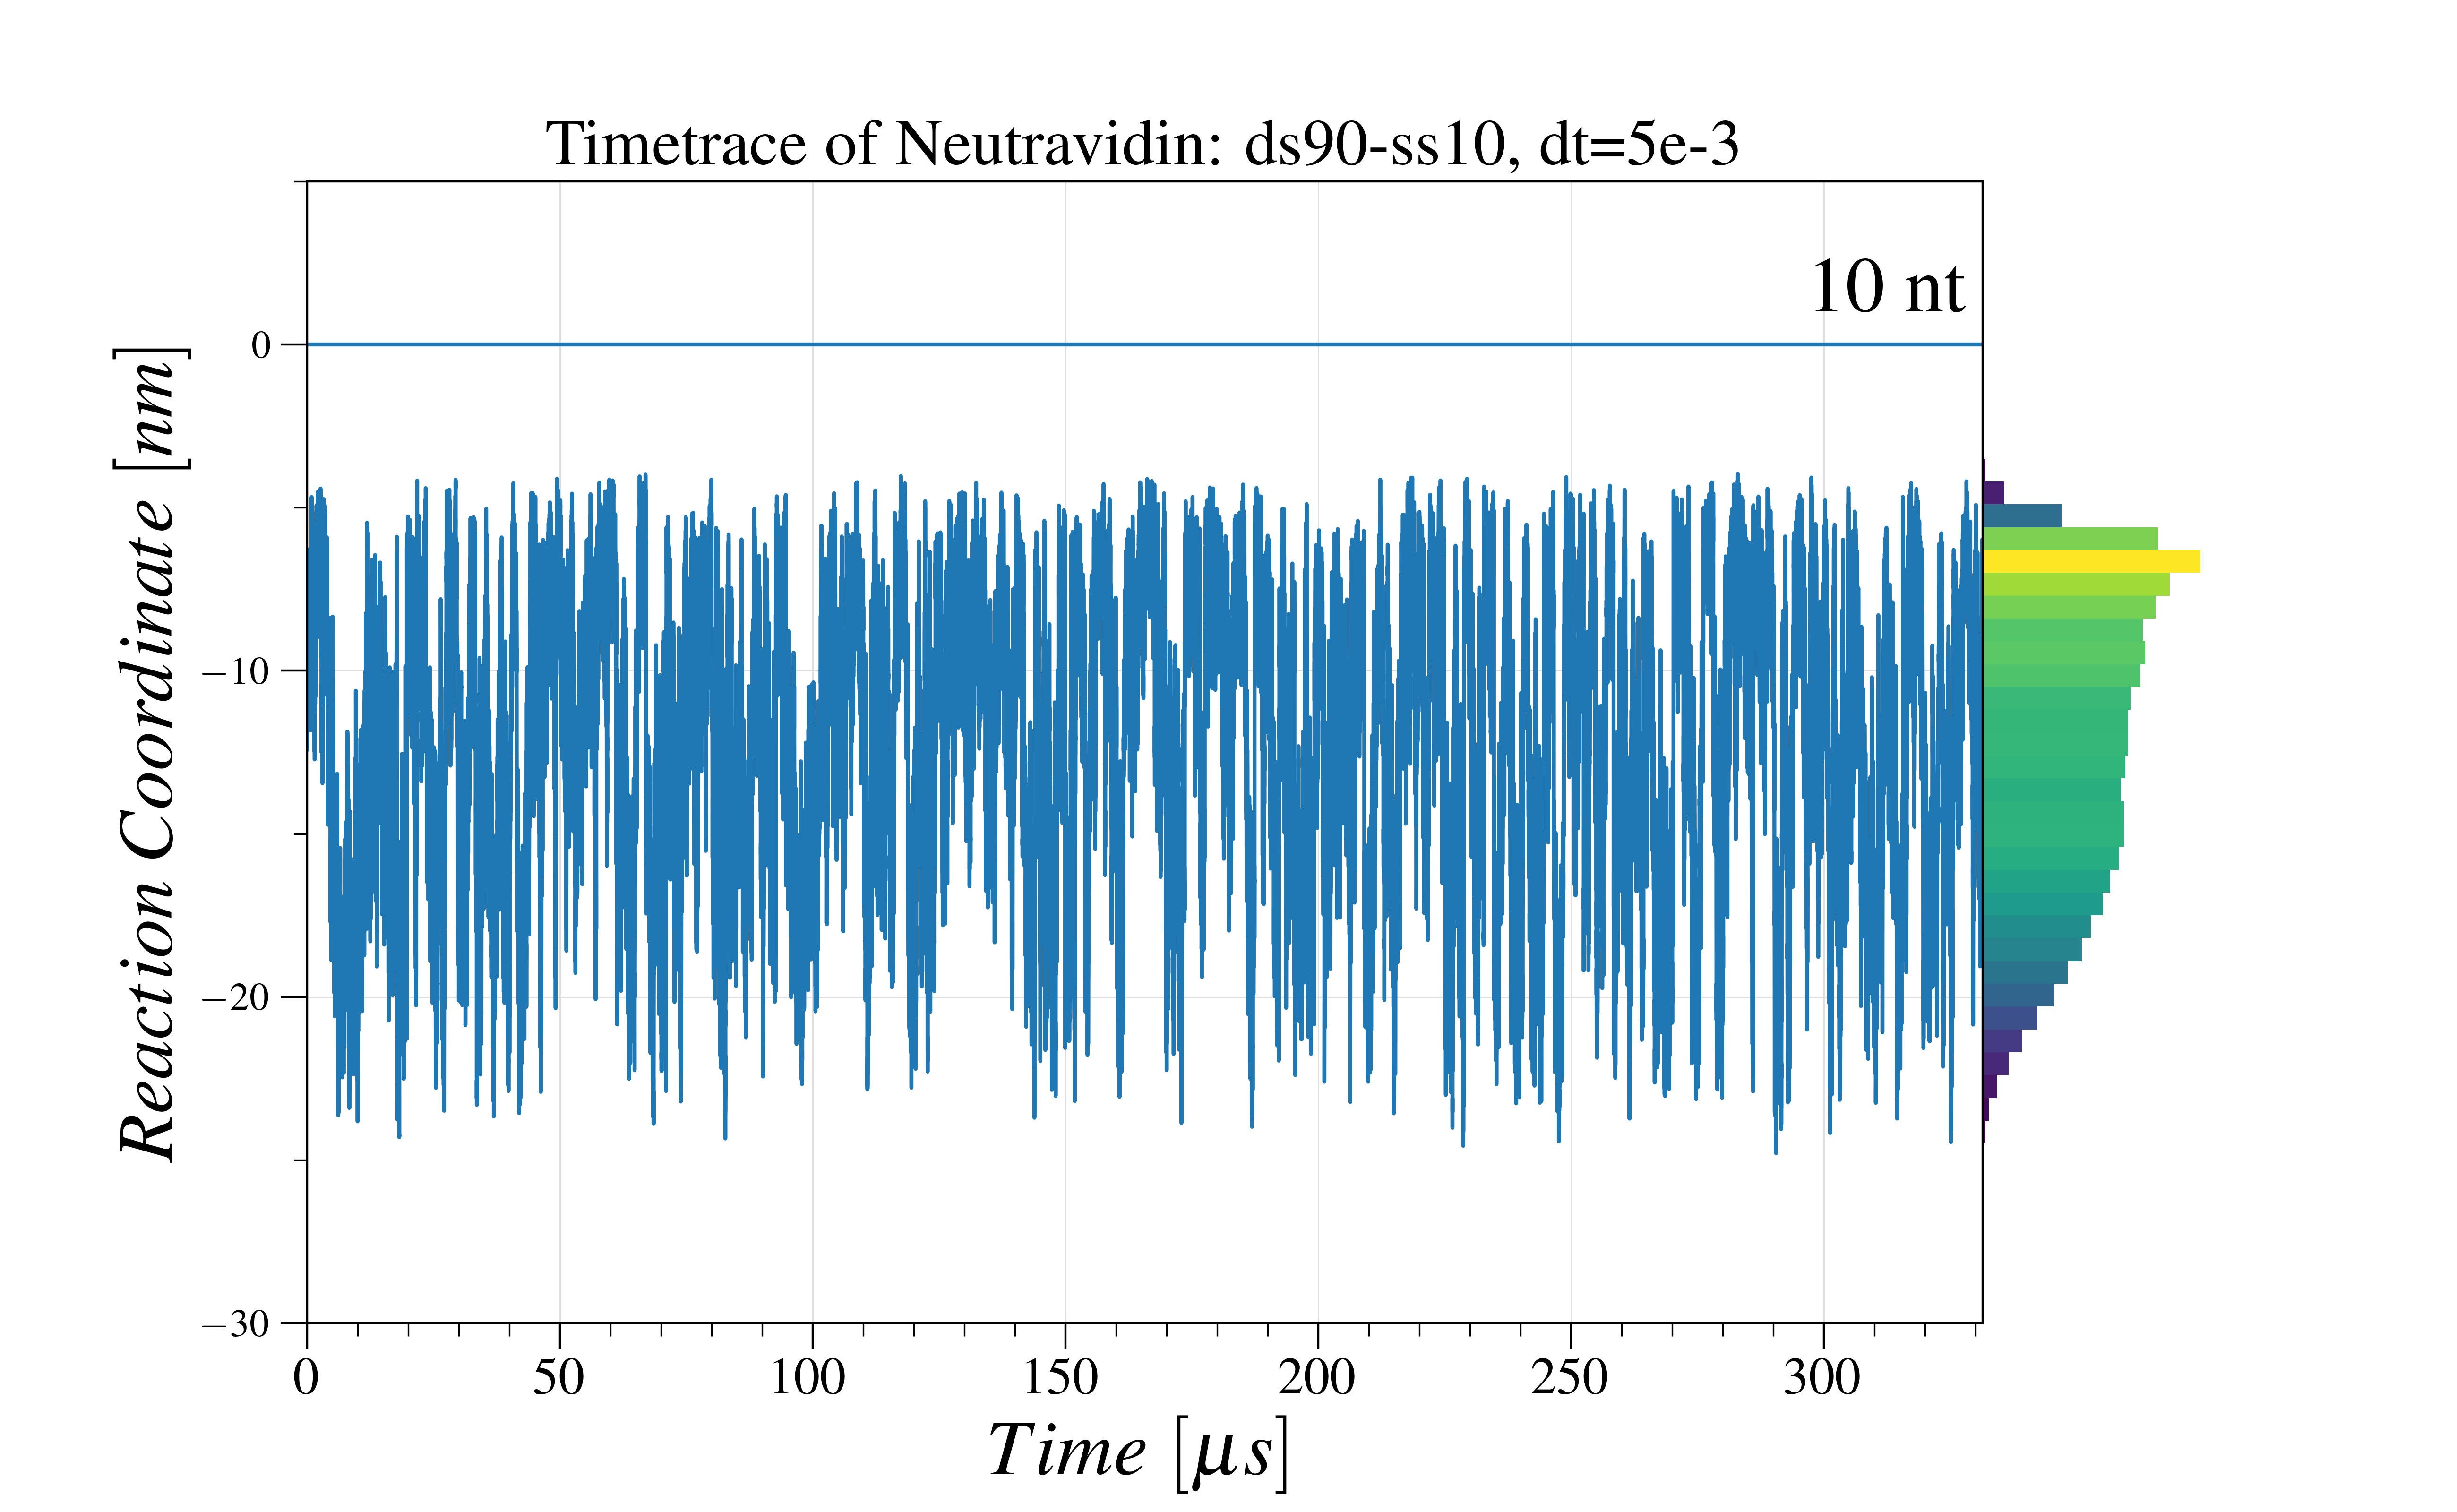
\includegraphics[width=.95\linewidth,valign=t]{Figures/MR-90.png}
  \end{subfigure}%
  \adjustbox{minipage=1.3em,valign=t}{}%
  \hspace{.3cm}
  \begin{subfigure}[t]{\dimexpr.21\linewidth-1.3em\relax}
  \centering
  \vspace{-0.5cm}
  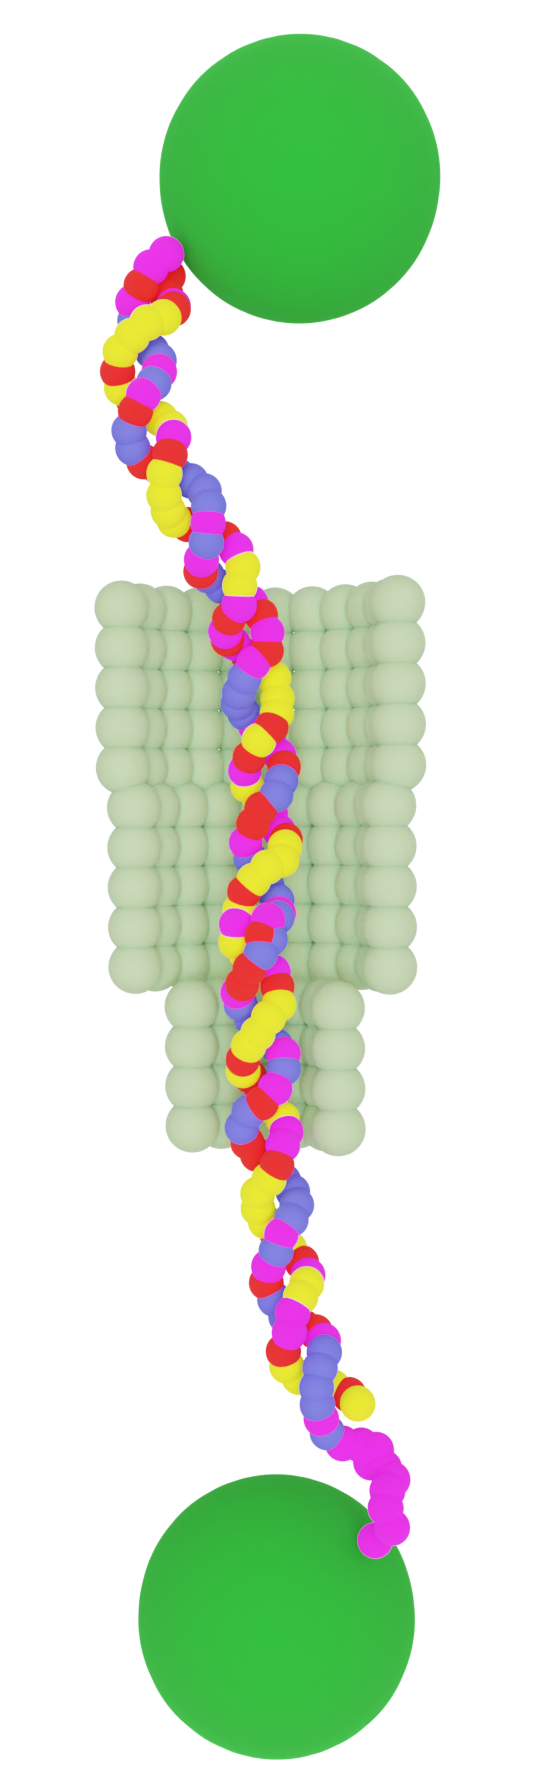
\includegraphics[width=.4\linewidth,valign=t]{Figures/Rotaxane-90.png}
  \end{subfigure}
  \label{fig:test}
  \end{centering}

  \vspace{.4cm}

  \begin{centering}
  \adjustbox{minipage=1.3em,valign=t}{}%
  \begin{subfigure}[t]{\dimexpr.3\linewidth-1.3em\relax}
  \centering
  \vspace{0.15cm}
  \hbox{\hspace{0.35cm}
  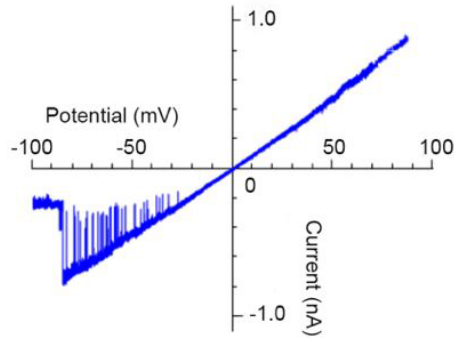
\includegraphics[width=1.05\linewidth,valign=t]{Figures/IV-80.png}}
  \end{subfigure}%
  \adjustbox{minipage=1.3em,valign=t}{}%
  \hspace{-0.5cm}
  \begin{subfigure}[t]{\dimexpr.46\linewidth-1.3em\relax}
  \centering
  \hbox{\hspace{0.56cm}
  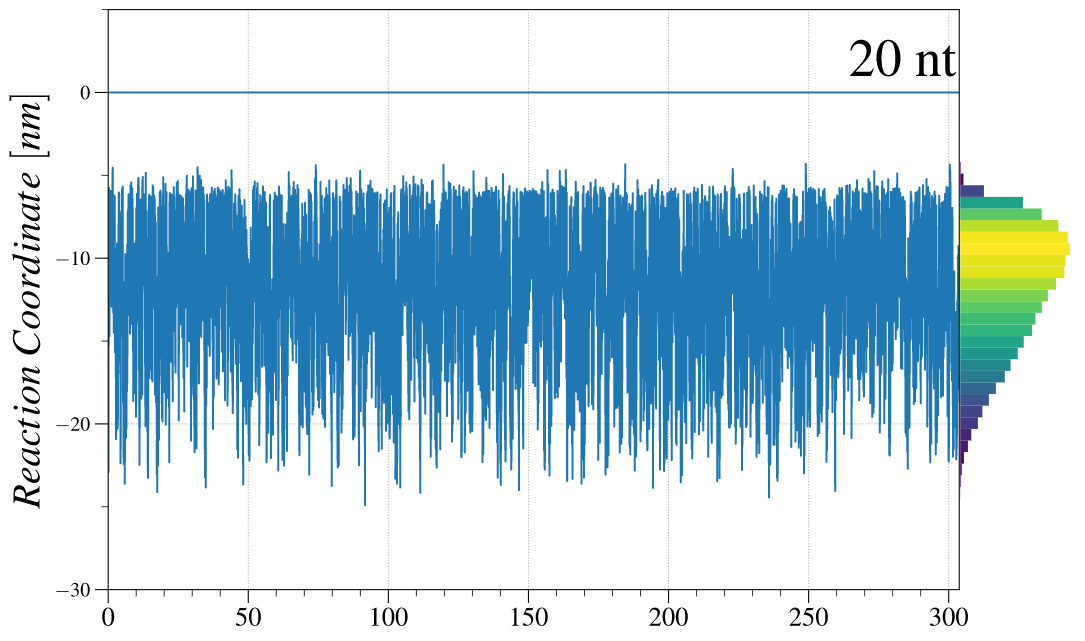
\includegraphics[width=.95\linewidth,valign=t]{Figures/MR-80.png}}
  \end{subfigure}%
  \adjustbox{minipage=1.3em,valign=t}{}%
  \hspace{.5cm}
  \begin{subfigure}[t]{\dimexpr.21\linewidth-1.3em\relax}
  \centering
  \vspace{-0.5cm}
  \hspace{-0.4cm}
  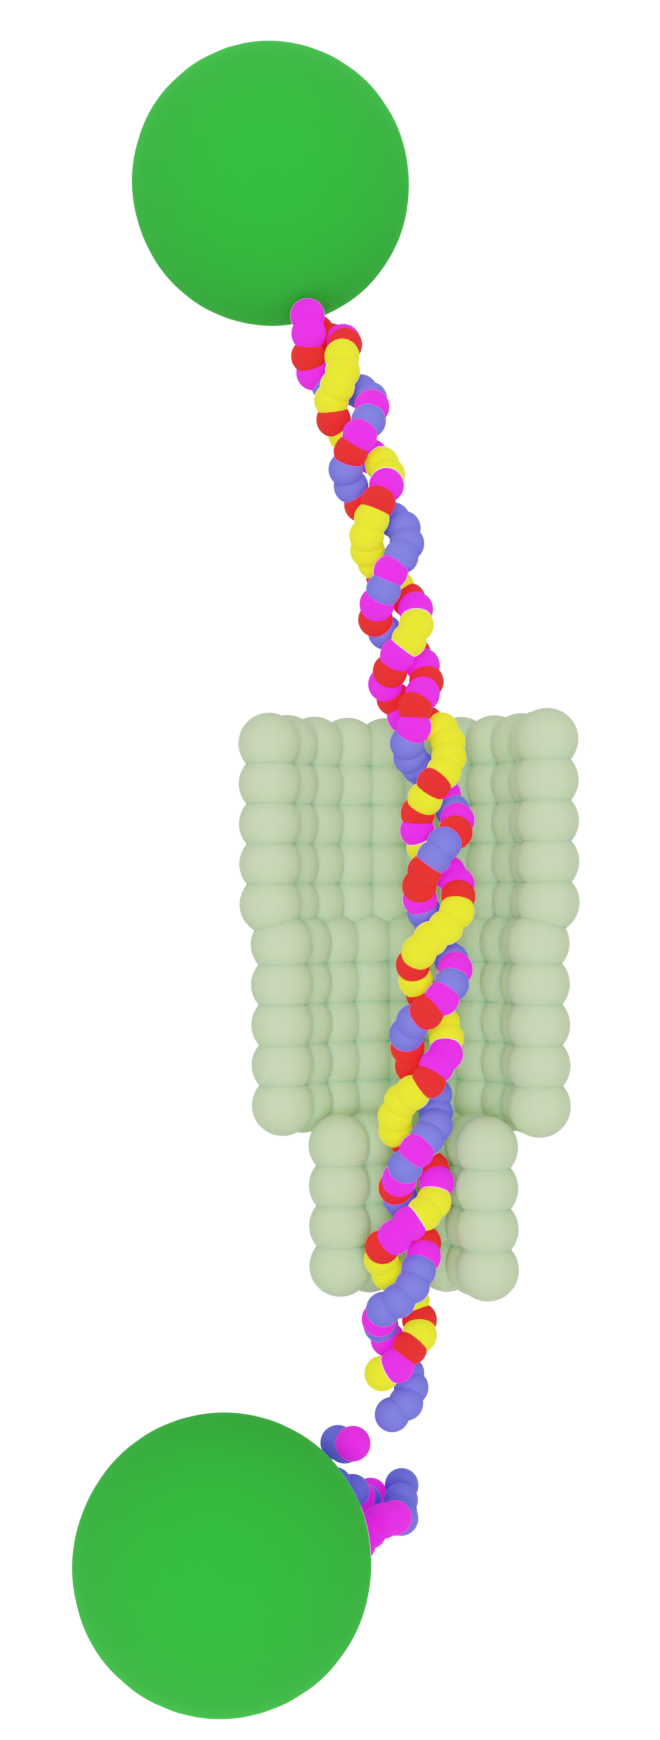
\includegraphics[width=.5\linewidth,valign=t]{Figures/Rotaxane-80.png}
  \end{subfigure}
  \label{fig:test}
  \end{centering}

  \vspace{.25cm}

  \begin{centering}
  \adjustbox{minipage=1.3em,valign=t}{}%
  \begin{subfigure}[t]{\dimexpr.3\linewidth-1.3em\relax}
  \centering
  \vspace{0.2cm}
  \hbox{\hspace{-0.0cm}
  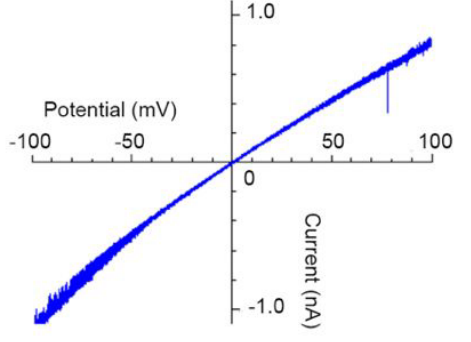
\includegraphics[width=1.05\linewidth,valign=t]{Figures/IV-70.png}}
  \end{subfigure}%
  \adjustbox{minipage=1.3em,valign=t}{}%
  \begin{subfigure}[t]{\dimexpr.46\linewidth-1.3em\relax}
  \centering
  \hbox{\hspace{0.0cm}
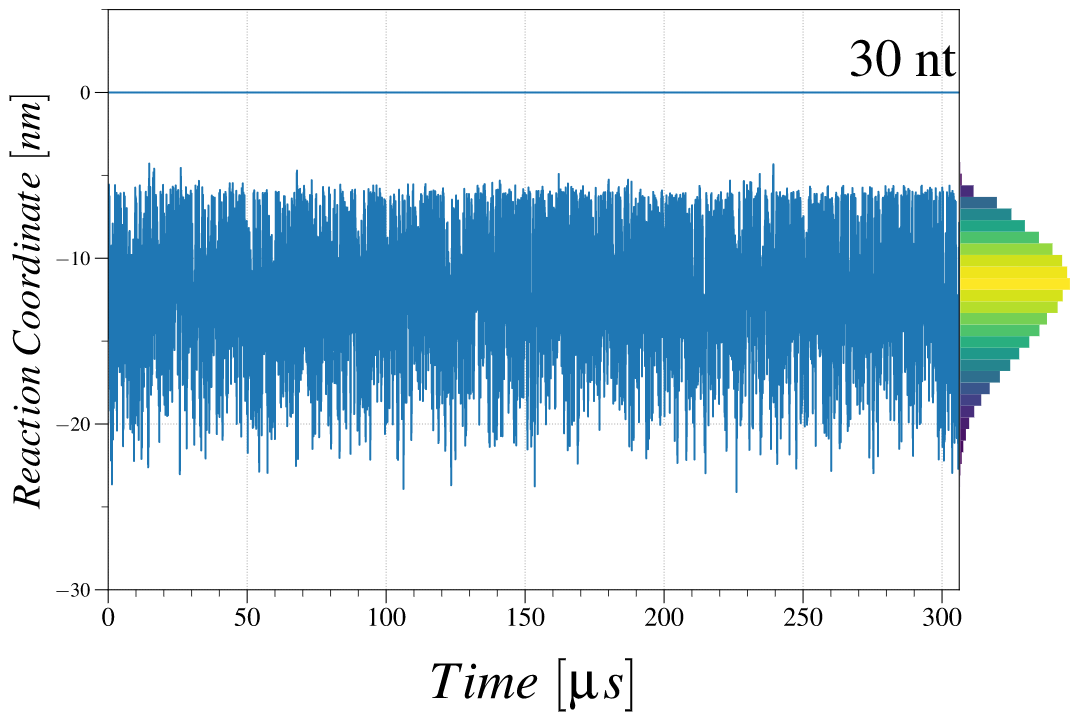
\includegraphics[width=.95\linewidth,valign=t]{Figures/MR-70.png}}
  \end{subfigure}%
  \adjustbox{minipage=1.3em,valign=t}{}%
  \hspace{0.5cm}
  \begin{subfigure}[t]{\dimexpr.21\linewidth-1.3em\relax}
  \centering
  \vspace{-0.6cm}
  
\includegraphics[width=.35\linewidth,valign=t]{Figures/Rotaxane-70.png}
  \end{subfigure}
  \caption[short lof/lot caption]{\linespread{0.5}{\small Analysis results for different
      variations of the mixed rotaxane. From top to bottom each horizontal set of figures
      corresponds to a mixed rotaxane with specific ssDNA length, ranging from $0\ nt$
      to $30\ nt$. (a) Experimental I-V traces obtained different variations of the mixed
      rotaxane. Both the current fluctuations and blockage are indicated with arrows.
      (b) Simulated reaction coordinate, defined in \ref{eq:reaction}, time traces of the
      of the trans-stopper. Here the blue line indicates the trans-entrance of the pore.
      On the right, the histograms corresponding to the trace is shown. (c) Snapshots of
      the rotaxane configurations taken from the simulations. Images for the I-V traces
      were taken from reference \cite{Bayoumi21}.}}
  \label{fig:mixedrotaxane}
  \end{centering}
\end{figure}

To interpret the observed characteristics in the I-V traces, molecular dynamics
simulation were performed of the mixed rotaxanes. The rotaxanes were simulated with no
bias, i.e. $0 mV$, to solely highlight the changes in the entropic effects. Quantifying
the conformational fluctuations of the rotaxane is done by tracing the trans-stopper
protein during the simulation using a reaction coordinate defined in our system. This
reaction coordinate, $X$, is determined as,
\begin{equation}
  X = \begin{cases}
        &z_0 + |\textbf{r} - \textbf{r}_{cis}|, \hspace{0.5cm} \textit{if on cis-side}\\
        &z, \hspace{2.5cm} \textit{if inside pore}\\
        &-|\textbf{r}|, \hspace{2.11cm} \textit{if on trans-side}
      \end{cases}
      \label{eq:reaction}
\end{equation}

defining a reaction coordinate for every bead in the system. In this coordinate frame,
the z-axis is aligned with the symmetry axis of the nanopore, placing the origin of
the coordinate system at center of the pore's trans-entrance. With respect to this
coordinate system, the center of pore's cis-entrance is located at $r_{cis} = (0,0,z_0)$.


In Figure \ref{fig:mixedrotaxane}b, the measured time trace of the $X$-coordinate of the
trans-stopper is presented for each mixed rotaxane type.  The horizontal line indicates
the origin of the reaction coordinate, representing the trans-entrance of the pore.
Observe that the trans-stopper is kept in the trans-reservoir by the repulsive boundary,
resulting in a negative $X$. On the right side of these time traces graphs, the
corresponding $X$-histograms are presented, indicating the positional distribution of
the trans-stopper during the simulations. It should be noted that the time traces are not
obtained from one continuous simulation, but rather aggregated from various independent
simulations performed in parallel, aiming to reduce the simulation time.

For the rotaxane fully composed of dsDNA, i.e. $0nt$, a uniform  $X$-histogram is found.
This result indicates free diffusion of the rotaxane within a bounded one dimensional
domain, namely the nanopore. As shown in the snapshot presented in Figure
\ref{fig:mixedrotaxane}c the rotaxane also fluctuates in the $x-y$ directions, however we
hypothesise that the one-dimensional diffusion effectively approximates the motion.
In the case where $10nt$ and $20nt$ are substituted into the composition of the rotaxane
a peak is observed in the $X$-histogram. This peak indicates a tendency of the
trans-stopper to move towards the entrance of the nanopore. This observation is in
agreement with the previously discussed I-V curves, since the presence of the stopper at
the pore entrance partially blocks the current flow. This tendency is driven by an
entropic force arising from the smaller ssDNA strand, being more easily captured in the
constriction of the pore compared to the large dsDNA strand.

Next, we observe that increasing the length of the ssDNA part of the mixed rotaxane
gradually shifts the histogram's peak further away from the pore entrance. Confining a
portion of the freely fluctuating ssDNA strand inside of the pore,
drastically reduces the number of available configurational microstates and thereby also
its entropy. This change in entropy induces an opposing entropic force.
An equilibrium configuration is found, when both the large dsDNA is kept outside of the
constriction, while allowing a maximal length of ssDNA strand to freely fluctuate outside
of the pore. These combined effects shift the peak of the distribution further away from
the pore entrance as the number of nucleotides is increased. An ever larger
electrophoretic force is required to sustain full pore blockage, which is why no blockage
is observed in the experiment's voltage range. The results found in these simulations are
in accordance with the corresponding simulations performed by Bayoumi et al., using
the bead-and-spring model.

\subsection{Mixed Rotaxane and 1D Confined Diffusion}

As the final part in our analysis of the mixed rotaxanes, the hypothesised free diffusive
behaviour of the $0nt$ mixed rotaxane is studied. The uniform distribution of the
$X$-histogram suggests that the rotaxane fluctuates predominantly vertically inside of
the pore like a rigid rod.  To study this diffusive behaviour, the mean square
displacements(MSD) of the trans-stopper is determined within a range of time
intervals.\footnote{The Tidynamics package was used for an efficient calculation of the
MSE. \cite{deBuyl2018}}
Calculating the MSD is done by utilising a rolling-window
analysis on the measured time trace. The MSD is an important quantity used to
characterise diffusive processes, since it allows us to verify whether an external force
influences the motion. For a particle that freely diffuses in a infinite one-dimensional
domain we know the MDS is given by
\begin{equation}
  \langle \Delta X^2 \rangle = 2 D t,
\end{equation}
here $D$ is the diffusion coefficient related to the particle. This simple linear
relation of the MSD is expected to only hold for our rotaxane at short times scales,
since the available domain is bounded. After a certain time the diffusive
motion of our rotaxane will cause the neutravidin protein stopper to collide with the
pore and interrupt the free diffusion. Resulting in the motion of the rotaxane being
described by one dimensional free diffusion with reflective boundary conditions.
From analytical calculations, presented in appendix A, we find
that the MSD for this motion can be expressed up to the second order as,
\begin{equation}
\langle \Delta X^2 \rangle = \frac{L^2}{6} - \frac{96}{\pi^4} e^{-\frac{D \pi^2t
}{L^2}},
\end{equation}
here $L$ is the length of the confined region, i.e. the hight of the pore. This model has
only one free fit parameter for which the value is fitted with our simulated data, the
result is presented in Figure \ref{fig:diff}.  From this we can conclude the $0nt$ mixed
rotaxane can be well described using the simple model of one dimensional confined
diffusion, confirming our postulation. This model predicts the diffusion coefficient of
the mixed rotaxane as, $69.08 \pm 0.02 \mu s^{-1}$, giving us an idea of the speed of the
rotaxane dynamics.
\begin{figure}[ht!]
\vspace{-0.3cm}
\begin{center}
  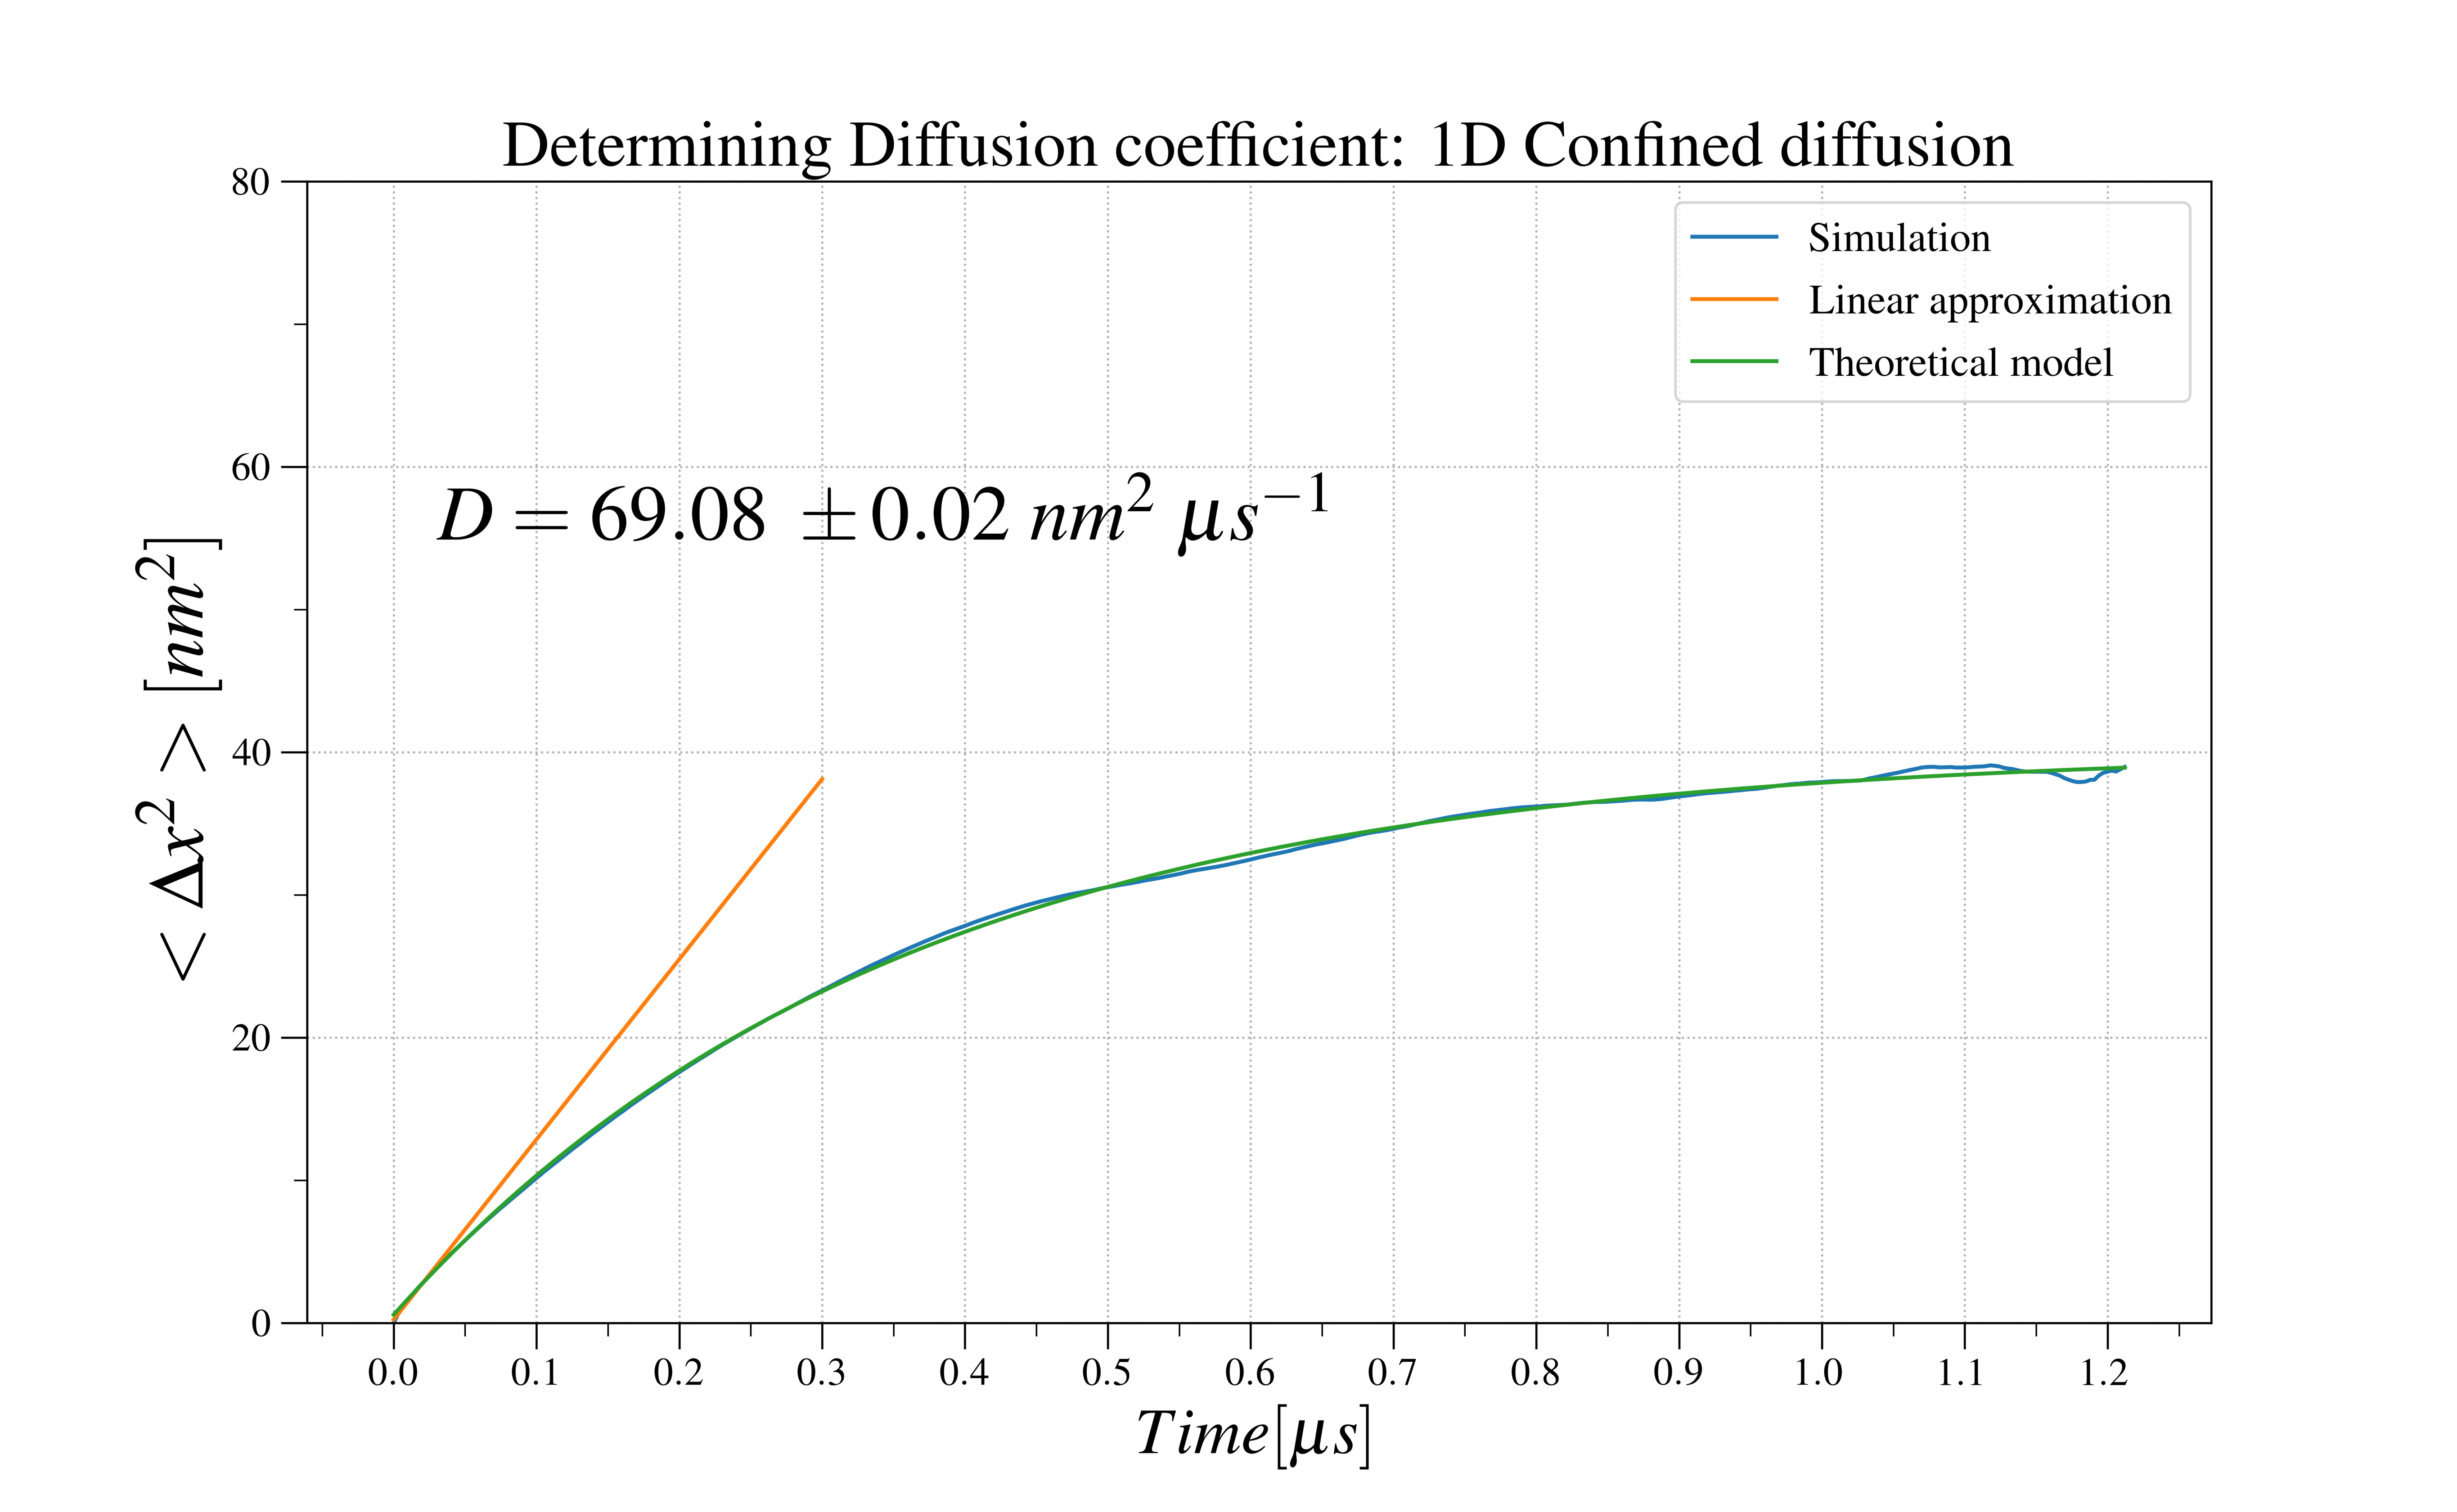
\includegraphics[width=0.7\textwidth]{Figures/MR-100-diff.png}
  \caption[Analysing the diffusive behaviour of the $0nt$ mixed
  rotaxane.]{\linespread{0.5}{\small Calculated mean squared displacement of the
  $0nt$ mixed rotaxane's motion for different time intervals. The data is fit to the
  obtained analytical models of free diffusion and confined diffusion. From the one
  parameter fit of the confined diffusion model, we obtain an accurate value for the
  diffusion coefficient of this motion: $ D = 69.08 \pm 0.02\ nm^2\ \mu s^{-1} $.}}
  \label{fig:diff}
\end{center}
\end{figure}
